\scanpage{27}
\uline{Special case} The one where $(xy)(zt)=0$ for any $x,y,z,t$, i.e.
\margin{[i.e. $(H^1)H^3=0$ in $H^4$ !]}
if the image of $\alpha:\bigwedge^2V\longrightarrow k\xi+W$ is \deleted{in} \unsure{an} isotropic subspace of $k(\xi)+W$.
\deleted{For example if $W\unsure{\neq0}$, in the algebraically closed case this is necessarily realized as follows : if $W$ is \inserted{of dimension} (odd), then one can}

$Q$ nondegenerate \unsure{being given|being given}, and suppose $W\neq0$, there exists (if $k$ \deleted{\unsure{then}} algebraically closed say) an isotropic line \inserted{$D$} in $k\xi+W$ which is not in $W$, and we shall take for $\alpha$ \deleted{a form} defined by a nondegenerate \inserted{alternating} bilinear \deleted{form}\inserted{map} \deleted{\unsure{on}} from $V\times V$ to $D$: then $\varphi$ will also be non-isotropic\ldots

\figure{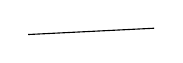
\begin{tikzpicture}\draw (0,0)--(1.6,0.08);\end{tikzpicture}}

More generally, consider the alternating 4-linear form $\chi$ defined by
\[
xyzt=\chi(x,y,z,t)\xi^2\qquad(x,y,z,t\in V)
\]
Then the \inserted{bilinear} form induced by the \inserted{form} $Q\oplus1$ (on $k\xi+V$) on $\bigwedge^2 V$ by $\alpha$, which defines a \deleted{form} linear form on
\diagram{\begin{tikzcd}[ampersand replacement=\&,column sep=large]
\operatorname{Sym}^2(\bigwedge^2V)\arrow[rr,bend right=18,"epimorphism"']\&\text{, factors through}\&\bigwedge^4V
\end{tikzcd}}
by means of $\chi$, and therefore the data are the following

a) $V$ vector space (of finite dimension) over $k$

\deleted{b) $\varphi:\bigwedge^2V\longrightarrow k$}

b) $\chi:\bigwedge^4V\longrightarrow k$, defining a symmetric bilinear form $\chi'$ on $\bigwedge^2V$

c) a vector space $\widetilde W$, with a \deleted{quadratic}\inserted{symmetric bilinear} form $\widetilde Q$, and a linear map
\[
\bigwedge^2V\xrightarrow{\alpha}\widetilde W
\]
compatible with $\chi',Q$ [we shall say that $\widetilde W,\widetilde Q$ is an \uline{extension} of the form $\chi'$]

d) an element $\xi$ of $\widetilde W$, such that $Q(\xi,\xi)=1$.

\uline{Nondegeneracy conditions}
\[
\left|\begin{array}{l}
Q\text{ nondegenerate}\\
\varphi(x,y)=Q(\alpha(x\wedge y),\xi)\text{ nondegenerate}
\end{array}\right.
\]
\mspage{26}
